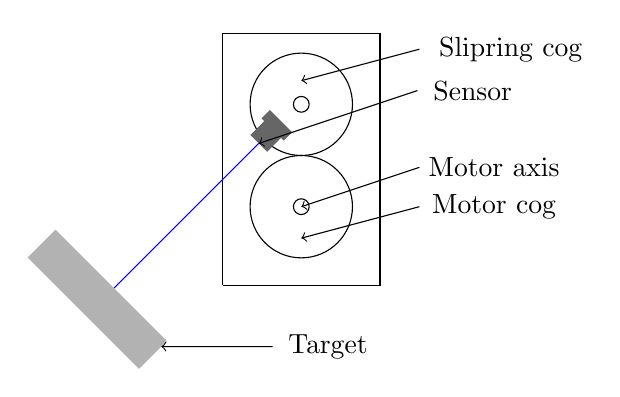
\begin{tikzpicture}[xscale=0.5, yscale=0.5]
\draw (0,0) -- (4,0) -- (4,6.4) -- (0,6.4) -- (0,0); %outre box
\draw (2,2) circle (1.3); %cog for motor
\draw (2,2) circle (0.2); % axis for motor
\draw (2,4.6) circle (1.3); %cog for slipring
\draw (2,4.6) circle (0.2); %axis for silp ring

%Sensor of the top cog
\fill[black!60!white, rotate=-45] (-2.3,4.0) rectangle (-1.5,3.7);
\fill[black!60!white, rotate=-45] (-2.2,3.2) rectangle (-1.6,3.8);
%beeam
\draw[blue, rotate=-45] (-1.9,3.2) -- (-1.9,-2);
%target
\fill[black!30!white, rotate=-45] (-4,-2) rectangle (0,-3);

%arrows
\draw[->, rotate=-45] (0,7)node[xshift=20] {Sensor} -- (-1.9,3.2);
\draw[->] (5,3)node[xshift=27] {Motor axis} -- (2.0,2.0) ;% motor axis
\draw[->] (5,2)node[xshift=27] {Motor cog} -- (2.0,1.2);% motor cog
\draw[->] (5,6)node[xshift=33] {Slipring cog} -- (2.0,5.2);% lidar cog
\draw[->, rotate=-45] (2,-0.2)node[xshift=20] {Target} -- (-0.0,-2.2);

\end{tikzpicture}